\documentclass[9pt]{beamer}
\usefonttheme[onlymath]{serif}
\usepackage[sfdefault]{roboto}
\usepackage[utf8]{inputenc}
\usepackage[T1]{fontenc}
\usepackage{styles/fluxmacros} 	% Define where theme files are located. 
\usefolder{styles}
\usetheme[style=red]{flux} % Available styles: asphalt, blue, red, green, gray 



\usepackage{graphicx}
\usepackage{amsmath}
\usepackage{amssymb}
\usepackage{amsfonts}
\usepackage{hyperref}

\title{Computerpraktikum Algebra}
\subtitle{Thema 4 - Graphen und Lie-Algebren}
\author{Pascal Bauer, Raphael Millon, Florian Haas}
\institute{Sommersemester 2020}
\date{\today}
\titlegraphic{assets/Empty.png}

\begin{document}

\titlepage 

\begin{frame}
 \frametitle{Table of contents}
 \tableofcontents
\end{frame}

\section{Theorie}
\begin{frame}{Theorie}
\begin{itemize}
\item Wir betrachten Dynkin-Diagramme und die daraus konstuierbaren Gruppen.
\item Dynkin-Diagramm sind spezielle Graphen, mit eventuell mehrfachen gerichteten Kanten.
\end{itemize}
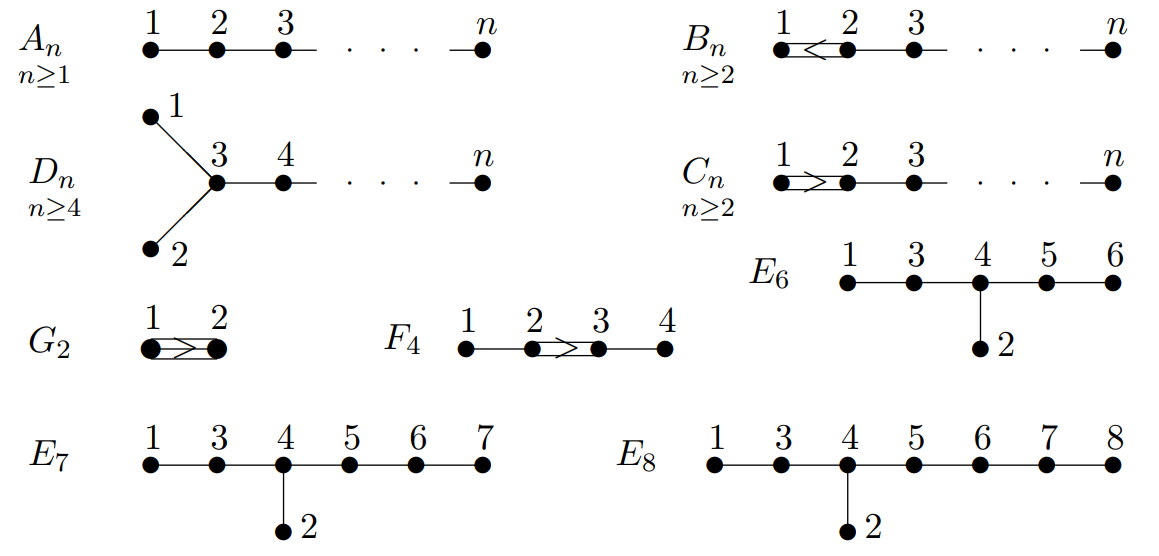
\includegraphics[width=\textwidth]{assets/dynkin.png}
\end{frame}

\begin{frame}{Theorie}
\begin{itemize}
\item Zu einem Graphen $\Gamma$ kann eine Matrix $A(\Gamma)=(a_{ij})_{1\leq i,j \leq n}$ wie folgt definiert werden:
\item \begin{enumerate}
	\item Setze $a_{ii} = 2$ auf der gesamten Diagonalen.
	\item Setze $a_{ij} = 0$, falls $i \neq j$ und die Ecken $i$ und $j$ nicht verbunden sind.
	\item Setze $a_{ij} = a_{ji} = -1$, falls $i \neq j$ und die Ecken $i$ und $j$ einfach verbunden sind.
	\item Setze $a_{ij} = -d, \ a_{ji} = -1$, falls $i \neq j$ und die Ecken $i$ und $j$ $d$-fach in Richtung $i$ verbunden sind.
	\end{enumerate}
\item Für $F_4$ ergibt sich zum Beispiel $$A(F_4)=\begin{pmatrix}2&-1&0&0\\-1&2&-1&0\\0&-2&2&-1\\0&0&-1&2\end{pmatrix}.$$
\item Somit kodieren sich $\Gamma$ und $A(\Gamma)$ gegenseitig.
\end{itemize}
\end{frame}

\begin{frame}{Theorie}
\begin{itemize}
\item Für festes $\Gamma$ definieren wir nun für $1 \leq i \leq n$ lineare Abbildungen gegeben durch $w_i(e_j) := e_j - a_{ij}e_i$ oder äquivalent $M_{\mathbb Q}(w_i) = I_n - E_{ii}A(\Gamma)$.
\item Da $M_{\mathbb Q}(w_i)^2 = I_n - 2E_{ii}A(\Gamma) + (E_{ii}A(\Gamma))^2 = I_n$ ist die Abbildung $w_i \in GL_n(\mathbb Q)$ und insbesondere diagonalisierbar mit Eigenwerten $\in \{-1,1\}$.
\item Jede Abbildung $w_i$ beschreibt also eine Spiegelung.
\item In unserem Projekt betrachteten wir die von allen $w_i$ erzeugte Gruppe $W = \langle w_1, \ldots, w_n \rangle \subseteq GL_n(\mathbb Q)$.
\item Zudem wird $\Phi = \{w(e_j) \mid w \in W, 1 \leq j \leq n\}$ berechnet. Insbesondere ist $\Phi$ genau dann endlich wenn auch $W$ endlich ist.
\end{itemize}
\end{frame}



\section{Showcase}
\begin{frame}{Showcase}
\begin{center}

\begin{tabular}{|c||c|c|c|c|c|c|c|c|}
\hline
Graph&$A_1$ & $A_2$ & $A_3$&$ A_4$ & $A_5$ & $A_6$& $A_7$ & $A_8$\\
\hline
$|\Phi|$ & 2 & 6 & 12 & 20 & 30 & 42 & 56 & 72\\
\hline
$|W|$ & 2&6&24&120&720&5040&40320&362880 \\
\hline
\hline
Graph&$-$ & $B_2$ & $B_3$&$ B_4$ & $B_5$ & $B_6$& $B_7$ & $B_8$\\
\hline
$|\Phi|$ & - & 8 & 18 & 32 & 50 & 72 & 98 & 128\\
\hline
$|W|$ & -&8&48&384&3840&46080&645120&10321920 \\
\hline
\hline
Graph&$-$ & $C_2$ & $C_3$&$ C_4$ & $C_5$ & $C_6$& $C_7$ & $C_8$\\
\hline
$|\Phi|$ & - & 8 & 18 & 32 & 50 & 72 & 98 & 128\\
\hline
$|W|$ & -&8&48&384&3840&46080&645120&10321920 \\
\hline
\hline
Graph&$-$ & $-$ & $-$&$D_4$ & $D_5$ & $D_6$& $D_7$ & $D_8$\\
\hline
$|\Phi|$ & - & - & - & 24 & 40 & 60 & 84 & 112\\
\hline
$|W|$ & -&-&-&192&1920&23040&322560&5160960 \\
\hline
\hline
Graph&$-$ & $-$ & $-$&$-$ & $-$ & $E_6$& $E_7$ & $E_8$\\
\hline
$|\Phi|$ & - & - & - & - & - & 72 & 126 & 240\\
\hline
$|W|$ & -&-&-&-&-&51840&2903040&696729600\\
\hline
\hline
Graph&$-$ & $G_2$ & $-$&$F_4$ & $-$ & $-$& $-$ & $-$\\
\hline
$|\Phi|$ & - & 12 & - & 48 & - & - & - & -\\
\hline
$|W|$ & -&12&-&1152&-&-&-&-\\
\hline
\end{tabular}\\
\end{center}
\end{frame}
\section{Ausgesuchte Codebeispiele}
\begin{frame}{Codebeispiele}
Unser Code ist Open-Source verfügbar auf Github: \begin{center}\url{https://github.com/raphaelMi/computerpraktikum-algebra}\end{center}

Implementiert haben wir vier Funktionen:
\begin{itemize}
\item{\texttt{gmat(X, n)}}
\item{\texttt{glin(graph\_matrix)}}
\item{\texttt{gphi(linear\_function\_matrices)}}
\item{\texttt{gw(linear\_function\_matrices)}}
\end{itemize}
\end{frame}

\begin{frame}{Codebeispiele}{gmat}
\begin{center}
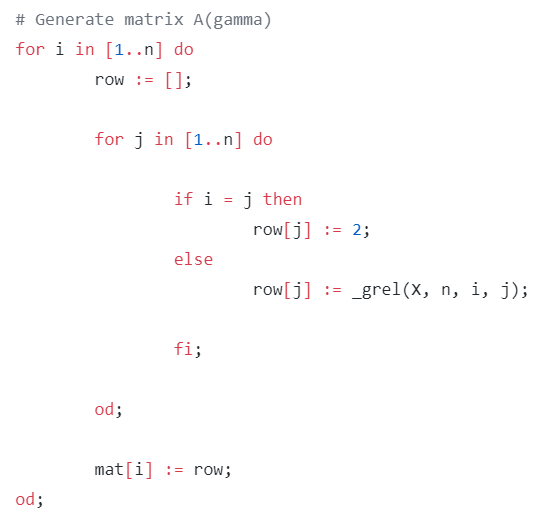
\includegraphics[scale=0.75]{assets/gmat_code.png}
\end{center}
\end{frame}

\begin{frame}{Codebeispiele}{glin}
\begin{center}
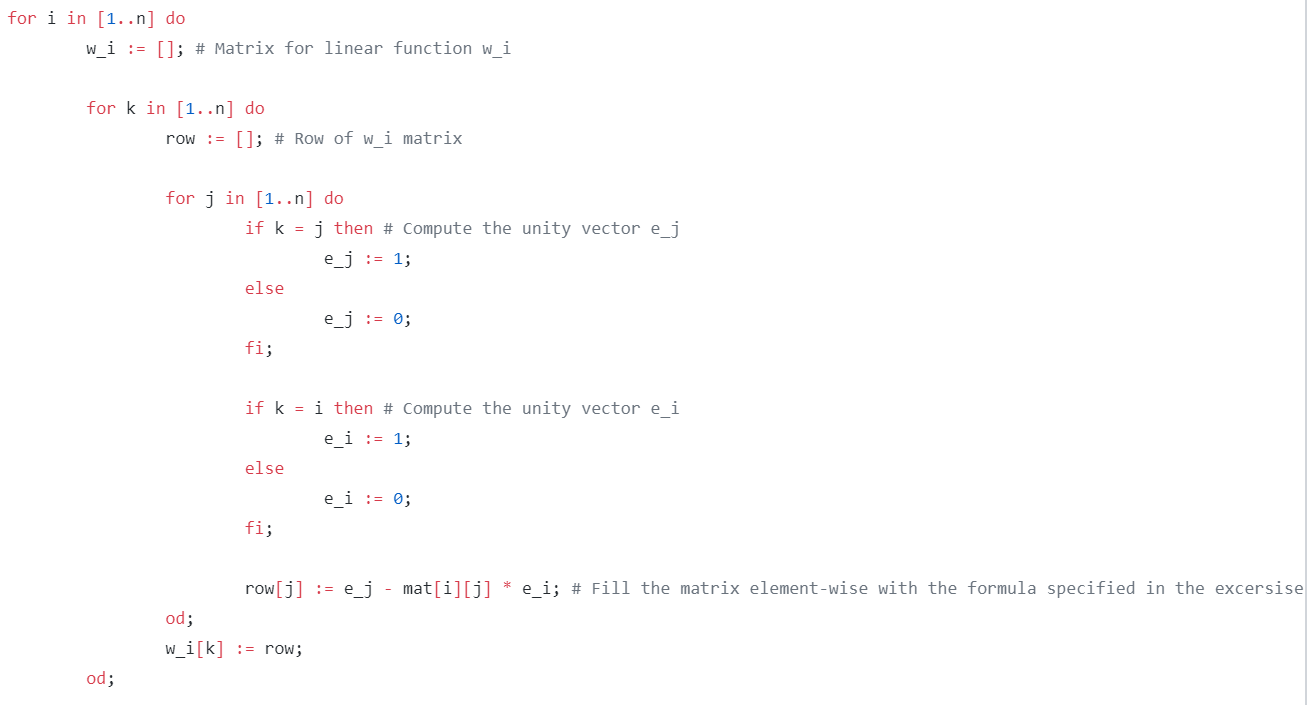
\includegraphics[scale=0.5]{assets/glin_code.png}
\end{center}
\end{frame}

\begin{frame}{Codebeispiele}{gphi}
\begin{center}
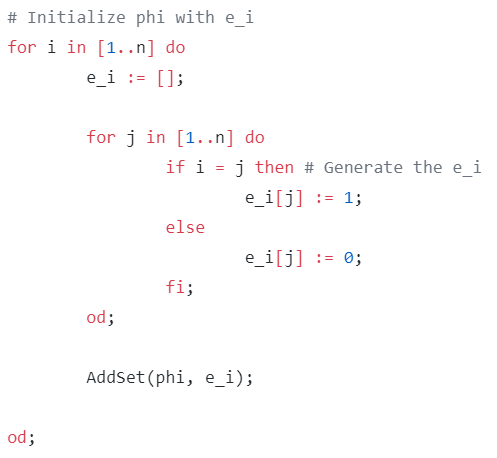
\includegraphics[scale=0.75]{assets/gphi_code_1.png}
\end{center}
\end{frame}

\begin{frame}{Codebeispiele}{gphi}
\begin{center}
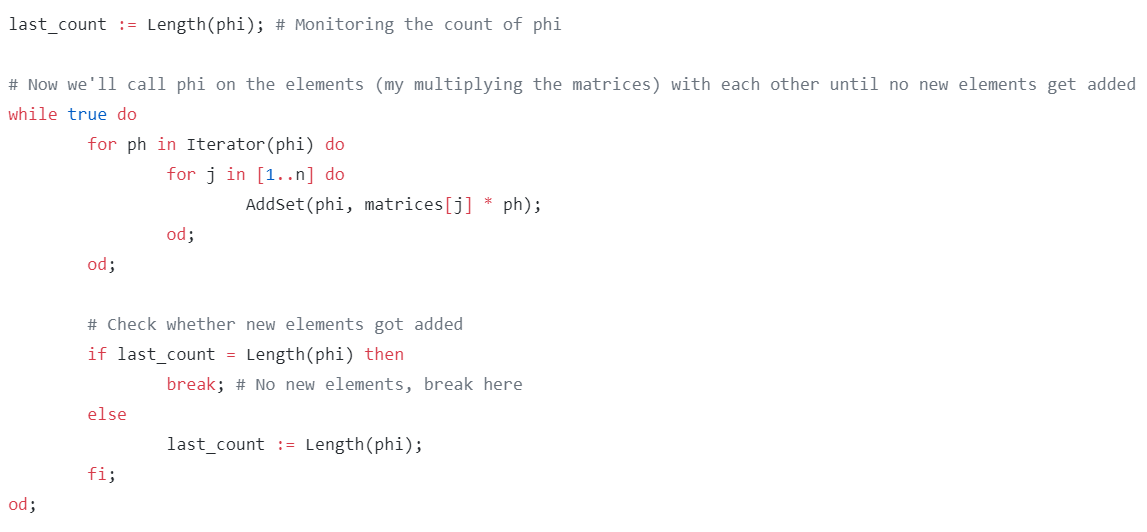
\includegraphics[scale=0.59]{assets/gphi_code_2.png}
\end{center}
\end{frame}

\begin{frame}{Codebeispiele}{gw}
\begin{center}
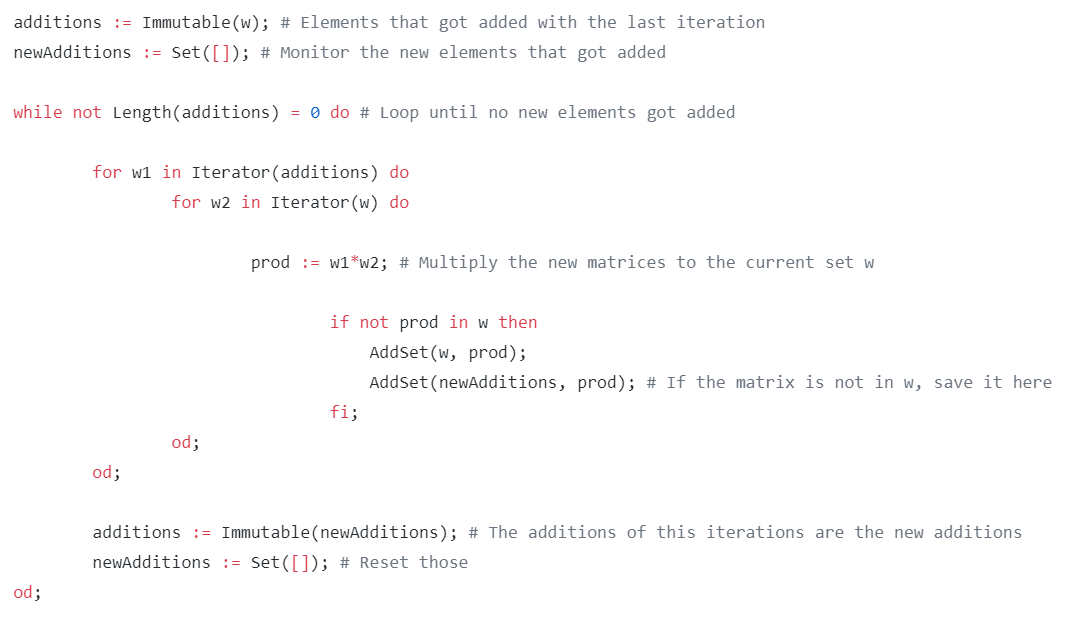
\includegraphics[scale=0.6]{assets/gw_code.png}
\end{center}
\end{frame}
\begin{frame}[fragile]{Fragen}{... und Antworten}
\begin{verbatim}
presentation_running := true;

while presentation_running do
	present();
od;

process_questions();
\end{verbatim}
\end{frame}
\end{document}